\documentclass[10pt, a4paper]{article}
% \usepackage[english]{babel}
\usepackage[brazilian]{babel}
\usepackage[utf8]{inputenc}
% \usepackage[T1]{fontenc}
\usepackage{lipsum}

% code
\usepackage{pythonhighlight}
\renewcommand{\lstlistingname}{Anexo} % Listing->Code
\usepackage{adjustbox}

% For subfigure use
\usepackage[font=small,labelfont=bf]{caption}
\usepackage{subcaption}

% Set page size and margins
% Replace `letterpaper' with`a4paper' for UK/EU standard size
\usepackage[a4paper,top=2cm,bottom=2cm,left=2cm,right=2cm,marginparwidth=2cm]{geometry}

% tabelas
\usepackage{array}
\usepackage{tabularx}
\usepackage{booktabs}

\usepackage{float}

% Useful packages
\usepackage{amsmath}
\usepackage{enumerate}

\usepackage{graphicx}
\usepackage[colorlinks=true, allcolors=blue]{hyperref}
\usepackage{cleveref}
%\usepackage[notransparent]{svg}
\newcommand{\crefrangeconjunction}{--}


\begin{document}

\def\TITLE{Trabalho 02}
\def\DISCIPLINE{MEC 2403 - Otimização e Algoritmos para Engenharia Mecânica}
\def\PROFESSOR{Ivan Menezes}
\def\AUTHOR{Pedro Henrique Cardoso Paulo}
\def\CONTACT{pedrorjpaulo.phcp@gmail.com}
\def\DATE{junho de 2023}

\title{\textbf{\TITLE} \\ \DISCIPLINE}
\author{\AUTHOR}
\date{\DATE}

\begin{titlepage}
      \begin{center}
          \vspace*{1cm}

          \Huge
          \textbf{\TITLE}

          \vspace{0.5cm}
          \LARGE
          \DISCIPLINE

          \vspace{1.5cm}

          \textbf{\AUTHOR \\ {\tt \CONTACT}}

          \vfill
          Professor: \PROFESSOR

          \vspace{0.8cm}

          
\includegraphics[width=0.2\textwidth]{../general/puc.jpg}

          \Large
          Departamento de Engenharia Mecânica\\
          PUC-RJ Pontifícia Universidade Católica do Rio de Janeiro\\
          \DATE

      \end{center}
  \end{titlepage}

\maketitle

\section{Introdução}

\subsection{Objetivos}

Esse é o entregável da \TITLE \ da disciplina \DISCIPLINE. Esse trabalho tem como objetivos:

\begin{enumerate}
  \item Expandir os métodos de otimização sem restrição (OSR) implementados na \href{https://github.com/prj-phcp/MEC2403_Activities/blob/master/Lista2/Lista2.pdf}{Lista 02} para a \
  tarefa de otimização com restrição (OCR)
  \item Implementar métodos de penalidade e barreira para restrições
  \item Realizar visualização dos resultados finais
\end{enumerate}

Para atingir esse objetivo, este trabalho consistirá na realização de dois exercícios. O primeiro consistirá na aplicação dos
métodos de otimização a duas funções distintas, sendo a primeira quadrática e a segunda não. O segundo exercício consistirá 
na solução de um problema de inspiração física, capaz de ser solucionado pelo método dos elementos finitos.

\subsection{Links úteis}\label{links}

Nesta seção são listados alguns links e referências úteis para se entender o trabalho desempenhado.

\begin{enumerate}
  \item \href{https://web.tecgraf.puc-rio.br/~ivan/MEC2403/ProgMatematica_VazPereiraMenezes-Ago2012.pdf}{Apostila de programação matemática da disciplina}
  \item \href{https://github.com/prj-phcp/MEC2403_Activities}{GitHub usado para essa disciplina}
  \item \href{https://github.com/prj-phcp/MEC2403_Activities/blob/master/Trabalho2/Trabalho2.ipynb}{Notebook com o código para as figuras desse relatório}
  \item \href{https://github.com/prj-phcp/MEC2403_Activities/blob/master/Trabalho2/Derivadas.ipynb}{Notebook com o código para derivação simbólica das funções mais complexas}
  \item \href{https://github.com/prj-phcp/MEC2403_Activities/blob/master/packages}{Pasta com os códigos a serem aproveitados em todas as listas}
\end{enumerate}

\section{Materiais e métodos}

Nesta seção serão descritos os principais métodos de otimização aplicados neste estudo, tal como detalhes de sua implementação
em código Python.

\subsection{Otimização sem restrição (OSR)}

Os métodos de otimização sem restrição, tal como os detalhes de suas implementações forma descritos no \href{https://github.com/prj-phcp/MEC2403_Activities/blob/master/Trabalho1/Trabalho1.pdf}{Trabalho 01}.
Para mais detalhes sobre esses métodos, referenciar o trabalho anterior.

\subsection{Otimização com restrições (OCR)}

O problema de otimização com restrições consiste em encontrar o mínimo de uma função que respeita um conjunto de restrições pré-determinadas. Um exemplo de problema
OCR é dado na equação \ref{eq:OCR}

\begin{equation}\label{eq:OCR}
  \begin{cases}
    \min f(\mathbf{x})\\
    h_i(\mathbf{x}) = 0, i\in 1, 2, 3, ... , n_h\\
    c_j(\mathbf{x}) \leq 0, j\in 1, 2, 3, ... , n_c
  \end{cases}\,.
\end{equation}

A solução deste problema passa por encontrar o mínimo da função $f$ respeitando as restrições de igualdade $h_i$ e de desigualdade $c_j$.
Embora técnicas analíticas como multiplicadores de Lagrange possam ser plicadas para esse conjunto de problemas, sua aplicação pode ser ineficiente
para aplicações numéricas, de modo que métodos como a Penlidade e a Barreira são preferíveis. A estrutura geral para aplicação desses métodos
segue a seguinte sequência de passos:


\begin{enumerate}
  \item Define-se os valores iniciais de $\mathbf{x}_0$, $r_p^0$ e $r_b^0$
  \item Aplica-se um método de OSR para uma função nova definida $\Phi(\mathbf{x}) = f(\mathbf{x}) + r_p^i p_p(\mathbf{x}) + r_b^i p_b(\mathbf{x})$,\
   determinando assim $\mathbf{x}_{i+1}$\label{item:otim}
  \item Para o ponto de resultado, calcula-se a métrica de erro $r_p^i p_p(\mathbf{x}_{i+1}) + r_b^i p_b(\mathbf{x}_{i+1})$
    \subitem Caso o erro seja inferior a uma tolerência, encerramos o processo e retornamos $\mathbf{x}_{i+1}$
    \subitem Caso contrário, atualizamos $r_p^{i+1} = \beta_p r_p^i$, $r_b^{i+1} = \beta_b r_b^i$ e retornamos para o item \ref{item:otim}. \
    Os valores de $\beta_p$ e $\beta_b$ são constantes ao longo da solução
\end{enumerate}

Nas próximas seções serão descritos brevemente os métodos de Penalidade e Barreira.

\subsubsection{Método da Penalidade}

O método da Penalidade soma a função otimizadora o termo descrito na equação \ref{eq:penalidade}

\begin{equation}\label{eq:penalidade}
  p_p(\mathbf{x}) = \sum_i^{n_h}(h(\mathbf{x}))^2 + \sum_j^{n_c}(\max{(c(\mathbf{x}),0)})^2\,.
\end{equation}

Dentre as características principais desse método temos a convergência facilitada para pontos iniciais for da região viável 
(embora pontos internos possam também convergir) e uma tendência de decrescimento da função $p_p$ conforme o ponto se aproxima de atender
às restrições, o que demanda que $r_p^i$ tenha uma tendência de crescimento ao longo das iterações (i.e., $\beta_p > 1.0$). Tende a ser um método
estável, convergindo para um ponto de mínimo na maioria dos casos.

\subsubsection{Método da Barreira}

O método da Barreira soma a função otimizadora o termo descrito na equação \ref{eq:barreira}

\begin{equation}\label{eq:barreira}
  p_b(\mathbf{x}) = - \sum_j^{n_c}\frac{1}{c(\mathbf{x})}\,.
\end{equation}

As principais características desse método é sua aplicação únicamente em condições de contorno de inequação e o faato deste convergir apenas para
pontos iniciais dentro da região viável. Condições de igualdade podem ser aplicadas por meio do método de penalidade em casos de uso do método da barreira,
porém a necessidade de um ponto interno é essencial, havendo necessidade da criação de proteções de código para garantir que durante a busca linear não haja
possibilidade de um ponto fora da região viável. Como a tendência de $p_b$ é de crescimento perto da fronteira, devemos garantir que $r_b^i$ tenha tendência 
de decréscimo (i.e., $\beta_b < 1.0$).

\subsection{Implementação}

Em adição aos módulos já desenvolvidos e exemplificados no \href{https://github.com/prj-phcp/MEC2403_Activities/blob/master/Trabalho1/Trabalho1.pdf}{Trabalho 01},
foram elaborados os seguintes módulos ccomplementares:


\begin{itemize}
  \item {\tt \href{https://github.com/prj-phcp/MEC2403_Activities/blob/master/packages/constraints.py}{constraints.py}}: Arquivo contendo as classes que simulam as
  restrições das funções. Herdam da classe {\tt SpecialFunction}
  \item {\tt \href{https://github.com/prj-phcp/MEC2403_Activities/blob/master/packages/constropt.py}{constropt.py}}: Arquivo que armazena o código para otimização
  com restrição. Recebem objetos das classes {\tt GenericOptimizer} e {\tt GenericStep}
\end{itemize}

Abaixo é apresentado o código do otimizador com restrição, elaborado para esse trabalho.

\begin{python}
class ConstrainedOptimizer:

def __init__(self, tol, max_iter=200, verbose=False):

    self.tol = tol
    self.max_iter = max_iter
    self.verbose = verbose
    self.clear_cache()

def clear_cache(self):
    self.cache_x = []
    self.iter = 0

def __call__(self, function:ConstrainedSpecialFunction, p_initial, optimizer:GenericOptimizer, step:GenericStep):

    self.clear_cache()
    function.start()
    x = p_initial
    errorflag = False
    while self.iter < self.max_iter:
        self.iter += 1
        if self.verbose: print(f'    Beginning iteration: {self.iter}')
        self.cache_x.append(x)
        da_original = step.get_da()
        da = step.get_da()
        x_new = optimizer(function, x, step)
        while not function.check_validity(x_new):
            da = da/10.0
            if self.verbose: print(f'       Original delta alpha too big. trying delta alpha = {da}')
            if da <= self.tol:
                errorflag = True
                break
            step.set_da(da)
            x_new = optimizer(function, x, step)
        step.set_da(da_original)
        x = x_new
        if self.verbose: print(f'    Ending iteration: {self.iter}. Final point: {x[0]},{x[1]}, loss: {function.loss(*x)}')
        if function.loss(*x) <= self.tol: 
            break
        if errorflag:
            print('    A step value inferior to the tolerance is needed in order to solve the problem. The iteractive process stopped. The best solution is returned')
            break
        function.step()
    self.cache_x.append(x)
    return x
\end{python}

\section{Resultados}

Todos os resultados apresentados foram gerados com códigos Python. A tolerância aplicada para a convergência OCR foi de $10^{-6}$, mas com o objetivo de facilitar
a convergência geral dos problemas, os códigos de OSR e busca linear utilizaram tolerâncias de $10^{-7}$ e $10^{-8}$, respectivamente. Todos os gradientes e hessianas
das funções e restrições foram calculados analíticamente e convertidos em funções Python com o auxílio da biblioteca {\tt sympy}.

\subsection{Questão 01}

Os resultados finais da Questão 01 foram sumarizados na Tabela \ref{tab:q1_results}. É possível ver que, para esse problema, todos os métodos de OSR retornaram essencialmente
o mesmo ponto final tanto para o método da Penalidade quanto o da Barreira. Além disso, os métodos de OSR para Penalidade e Barreira seguiram essencialmente o mesmo caminho,
com basicamente o memo número de passos, o que é esperado dado que todos os métodos de OSR devem, a cada busca de $\Phi$, retornar o mesmo ponto de mínimo.

\begin{table}[htpb]
  \centering
  \begin{tabular}{|l|c|c|c|c|c|c|c|}
    %\cline{2-7}
    \multicolumn{1}{c}{} %\vline
    & 
    \multicolumn{3}{c}{\textbf{Penalidade}} \vline
    & 
    \multicolumn{3}{c}{\textbf{Barreira}} \\%\vline \\
    \hline%\cline{2-5}
    \textbf{Método}
    &
    \textbf{Ponto de mínimo}
    & 
    $\mathbf{n}_{passos}$
    & 
    \textbf{t (s)}
    &
    \textbf{Ponto de mínimo}
    & 
    $\mathbf{n}_{passos}$
    & 
    \textbf{t (s)}
    \\
    Univariante        & $[0.942897, 0.889055]^T$ &  8 & 0.687 &  $[0.947491, 0.897739]^T$ &  13  & 1.475    \\
    Powell             & $[0.945580, 0.894121]^T$ &  8 & 0.500 &  $[0.945550, 0.894063]^T$ &  15  & 0.619    \\
    Steepest Descent   & $[0.945543, 0.894051]^T$ &  8 & 0.631 &  $[0.945652, 0.894255]^T$ &  14  & 1.617    \\
    Fletcher-Reeves    & $[0.945584, 0.894129]^T$ &  8 & 0.648 &  $[0.945592, 0.894145]^T$ &  13  & 1.307    \\
    Newton-Raphson     & $[0.945583, 0.894127]^T$ &  8 & 0.475 &  $[0.945583, 0.894126]^T$ &  15  & 1.729    \\
    BFGS               & $[0.945583, 0.894127]^T$ &  8 & 0.651 &  $[0.945584, 0.894127]^T$ &  15  & 0.482    \\
    \hline
  \end{tabular}
  \caption{Resumo dos resultados obtidos para a Questão 01}
  \label{tab:q1_results}
\end{table}

Três problemas específicos foram detectados na realização deste exercício: casos em que o método da barreira atingia pontos fora do domínio, casos em que Powell
retornava um vetor de busca nulo e casos em que métodos como o BFGS retornavam vetores inválidos por matriz singular. Os três casos foram tratados por meio da adição
de proteções no código para evitar a parada do processo e garantir que o ponto retornado sempre ficasse dentro do domínio. Vale resslatar que para este caso a maioria 
dos problemas ocorreu apenas no método da barreira.

A Figura \ref{fig:q1} apresenta os resultados em gráfico. Novamente, fica evidente que o caminho percorrido, independente do método OSR, foi extremamente similar.
Ressalta-se que a região viável nas figuras é marcada com cinza, para todas as restrições.


\begin{figure}[htpb]
  \centering
  \begin{subfigure}[b]{0.32\textwidth}
      \centering
      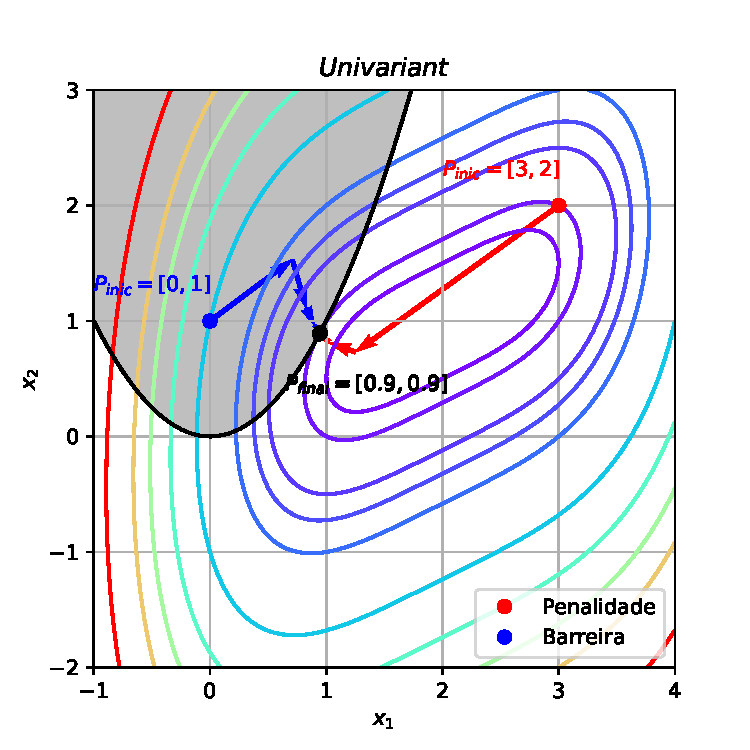
\includegraphics[width=\textwidth]{images/q1_Univariant.pdf}
      \caption{Univariante}
      \label{fig:q1_univariant}
  \end{subfigure}
  \hfill
  \begin{subfigure}[b]{0.32\textwidth}
    \centering
    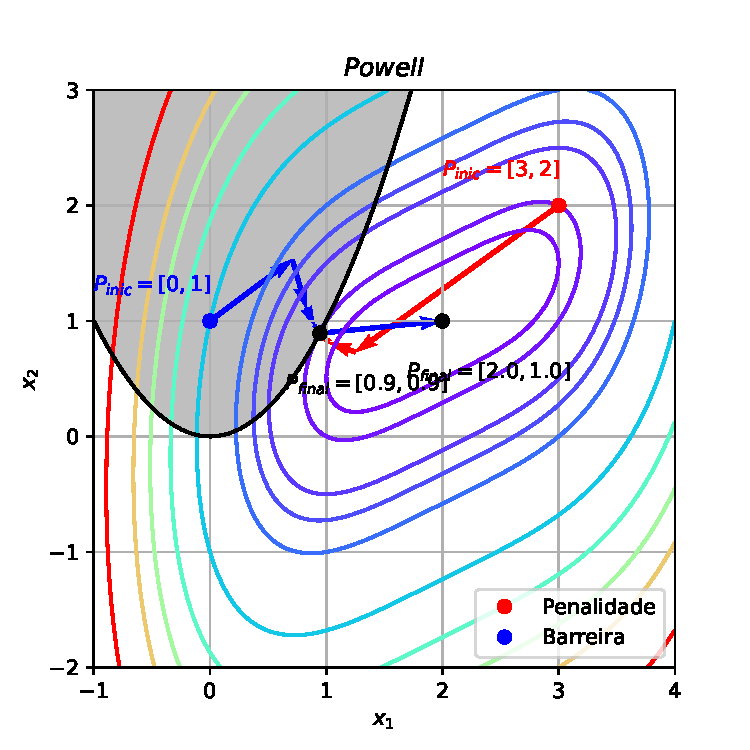
\includegraphics[width=\textwidth]{images/q1_Powell.pdf}
    \caption{Powell}
    \label{fig:q1_powell}
  \end{subfigure}
  \hfill
  \begin{subfigure}[b]{0.32\textwidth}
    \centering
    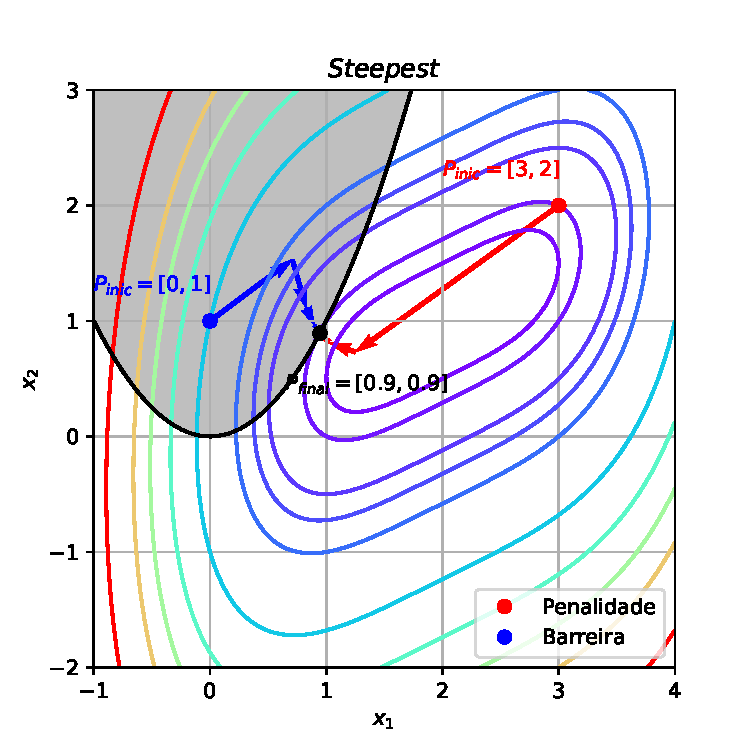
\includegraphics[width=\textwidth]{images/q1_Steepest.pdf}
    \caption{Steepest Descent}
    \label{fig:q1_steepest}
  \end{subfigure}
  \hfill
  \begin{subfigure}[b]{0.32\textwidth}
    \centering
    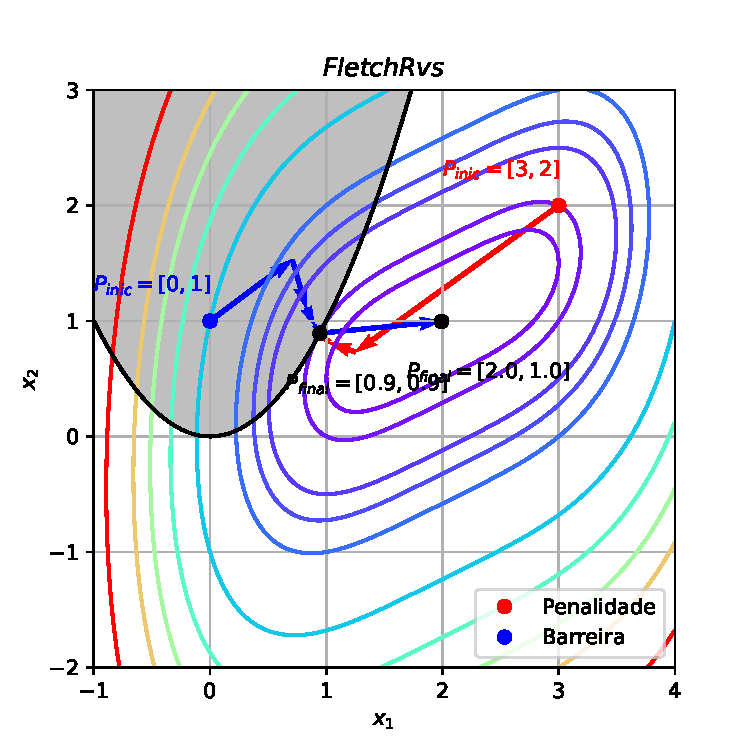
\includegraphics[width=\textwidth]{images/q1_FletchRvs.pdf}
    \caption{Fletcher-Reeves}
    \label{fig:q1_fletchrvs}
  \end{subfigure}
  \hfill
  \begin{subfigure}[b]{0.32\textwidth}
    \centering
    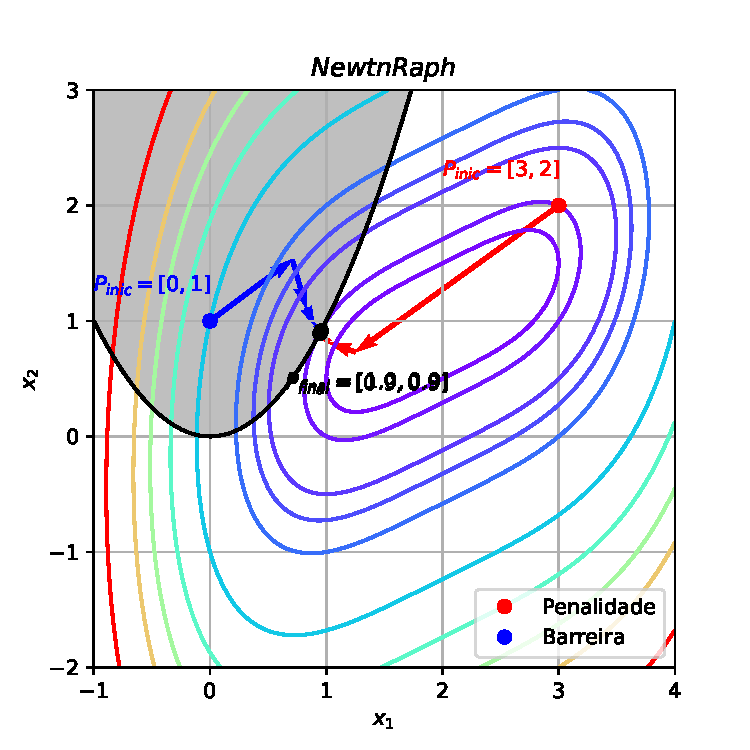
\includegraphics[width=\textwidth]{images/q1_NewtnRaph.pdf}
    \caption{Newton-Raphson}
    \label{fig:q1_newtnraph}
  \end{subfigure}
  \hfill
  \begin{subfigure}[b]{0.32\textwidth}
    \centering
    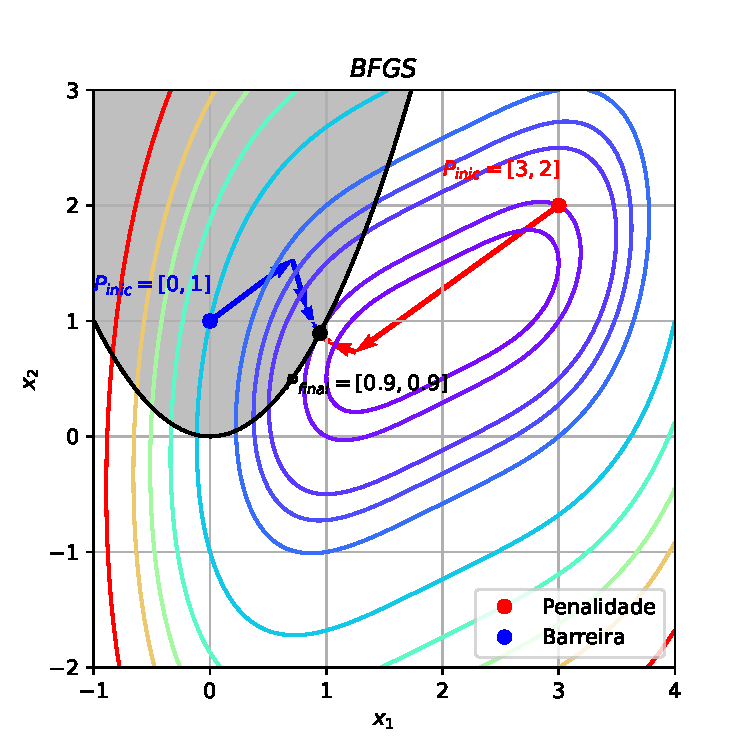
\includegraphics[width=\textwidth]{images/q1_BFGS.pdf}
    \caption{BFGS}
    \label{fig:q1_bfgs}
  \end{subfigure}
     \caption{Resultados gráficos para a Questão 01}
     \label{fig:q1}
\end{figure}


\subsection{Questão 02}

Os resultados obtidos para a Questão 02 são exibidos em forma tabular na Tabela \ref{tab:q2_results} e graficamente na Figura \ref{fig:q2}. As conclusões obtidas neste caso são similares
às obtidas na Questão 01.

\begin{table}[htpb]
  \centering
  \begin{tabular}{|l|c|c|c|c|c|c|c|}
    %\cline{2-7}
    \multicolumn{1}{c}{} %\vline
    & 
    \multicolumn{3}{c}{\textbf{Penalidade}} \vline
    & 
    \multicolumn{3}{c}{\textbf{Barreira}} \\%\vline \\
    \hline%\cline{2-5}
    \textbf{Método}
    &
    \textbf{Ponto de mínimo}
    & 
    $\mathbf{n}_{passos}$
    & 
    \textbf{t (s)}
    &
    \textbf{Ponto de mínimo}
    & 
    $\mathbf{n}_{passos}$
    & 
    \textbf{t (s)}
    \\
    Univariante        & $[1.878357, 20.236907]^T$ &  6 & 1.336 &  $[1.878355, 20.236914]^T$ &  15  & 2.902    \\
    Powell             & $[1.878357, 20.236907]^T$ &  6 & 1.087 &  $[1.878356, 20.236914]^T$ &  16  & 0.810    \\
    Steepest Descent   & $[1.878357, 20.236905]^T$ &  6 & 1.300 &  $[1.878355, 20.237137]^T$ &  15  & 3.074    \\
    Fletcher-Reeves    & $[1.878357, 20.236908]^T$ &  6 & 1.369 &  $[1.878357, 20.236927]^T$ &  15  & 2.710    \\
    Newton-Raphson     & $[1.878357, 20.236907]^T$ &  6 & 1.493 &  $[1.878357, 20.236908]^T$ &  16  & 3.068    \\
    BFGS               & $[1.878357, 20.236907]^T$ &  6 & 0.917 &  $[1.878357, 20.236914]^T$ &  16  & 0.860    \\
    \hline
  \end{tabular}
  \caption{Resumo dos resultados obtidos para a Questão 02}
  \label{tab:q2_results}
\end{table}

\begin{figure}[htpb]
  \centering
  \begin{subfigure}[b]{0.32\textwidth}
      \centering
      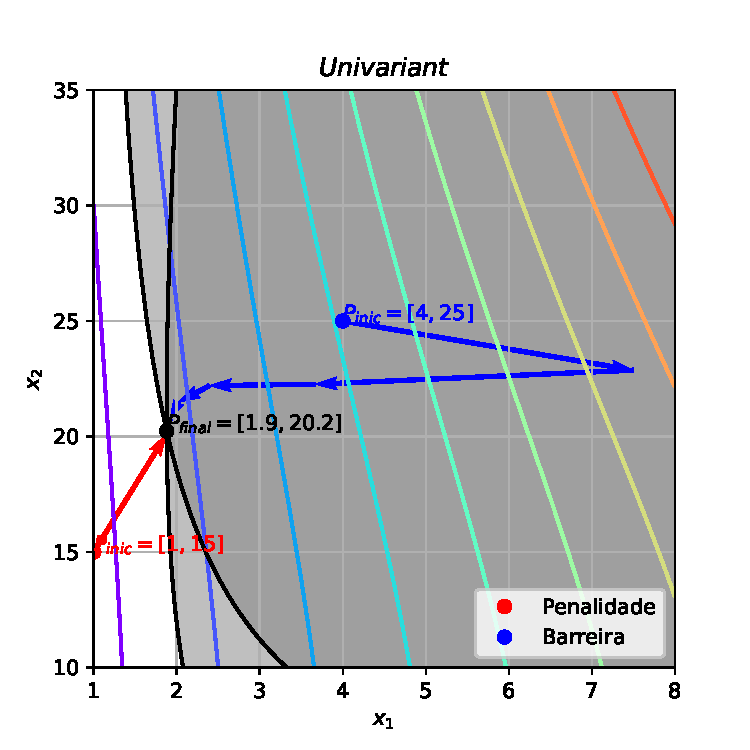
\includegraphics[width=\textwidth]{images/q2_Univariant.pdf}
      \caption{Univariante}
      \label{fig:q2_univariant}
  \end{subfigure}
  \hfill
  \begin{subfigure}[b]{0.32\textwidth}
    \centering
    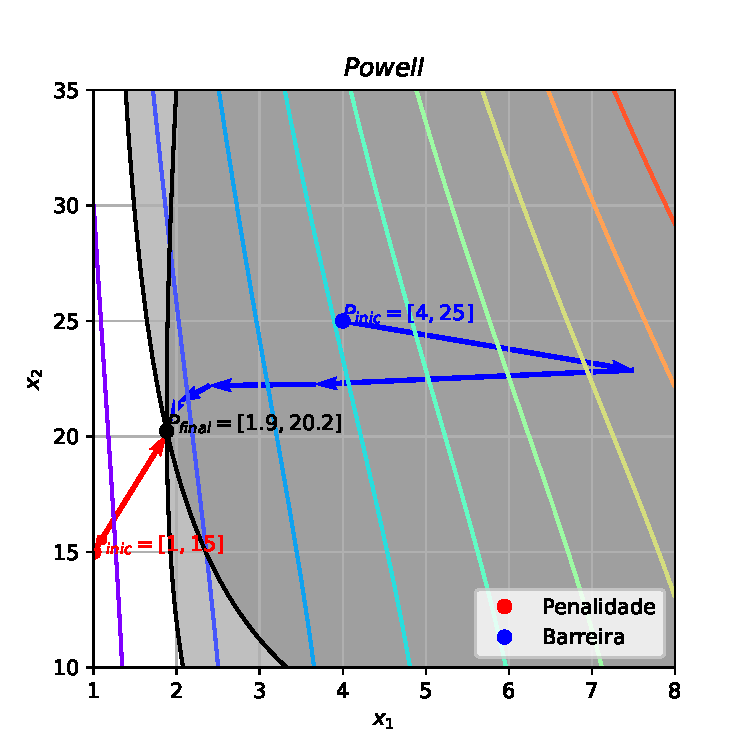
\includegraphics[width=\textwidth]{images/q2_Powell.pdf}
    \caption{Powell}
    \label{fig:q2_powell}
  \end{subfigure}
  \hfill
  \begin{subfigure}[b]{0.32\textwidth}
    \centering
    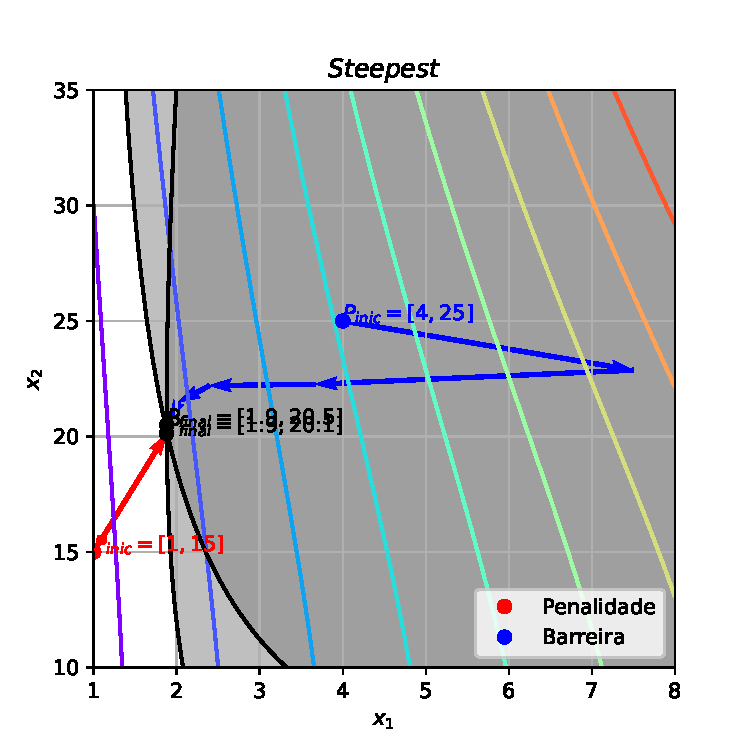
\includegraphics[width=\textwidth]{images/q2_Steepest.pdf}
    \caption{Steepest Descent}
    \label{fig:q2_steepest}
  \end{subfigure}
  \hfill
  \begin{subfigure}[b]{0.32\textwidth}
    \centering
    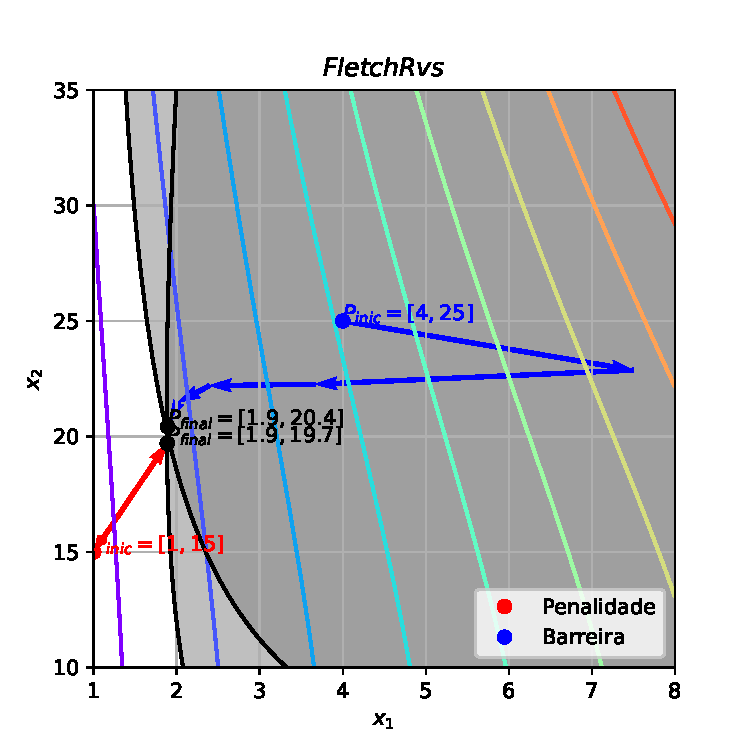
\includegraphics[width=\textwidth]{images/q2_FletchRvs.pdf}
    \caption{Fletcher-Reeves}
    \label{fig:q2_fletchrvs}
  \end{subfigure}
  \hfill
  \begin{subfigure}[b]{0.32\textwidth}
    \centering
    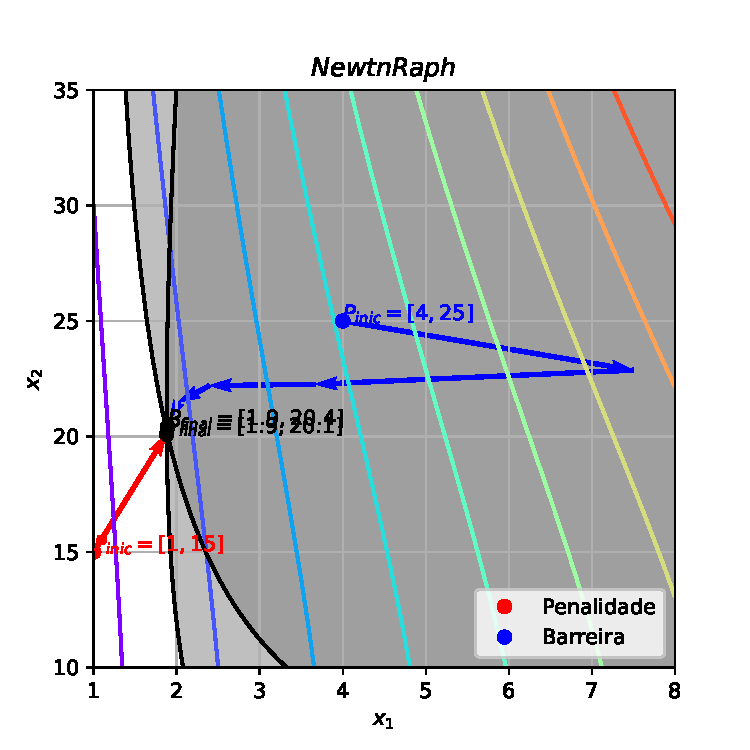
\includegraphics[width=\textwidth]{images/q2_NewtnRaph.pdf}
    \caption{Newton-Raphson}
    \label{fig:q2_newtnraph}
  \end{subfigure}
  \hfill
  \begin{subfigure}[b]{0.32\textwidth}
    \centering
    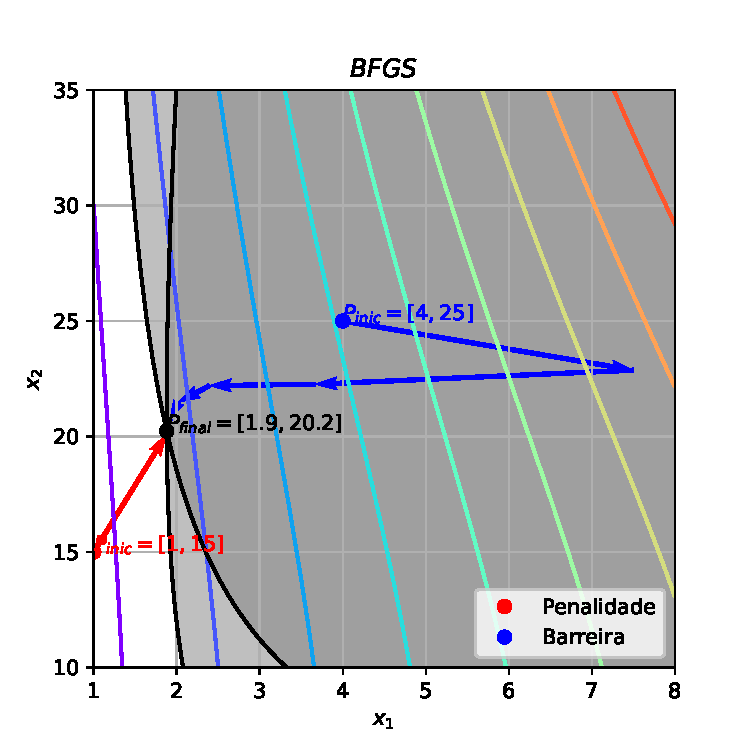
\includegraphics[width=\textwidth]{images/q2_BFGS.pdf}
    \caption{BFGS}
    \label{fig:q2_bfgs}
  \end{subfigure}
     \caption{Resultados gráficos para a Questão 02}
     \label{fig:q2}
\end{figure}

\newpage
As funções de restrição aplicadas nesse caso são mostradas a seguir. Cabe ressaltar que a formulação do problema foi retirada dos slides e material de aula, com derivadas analíticas
obtidas com a ajuda do {\tt sympy}.

\begin{python}
  cfs = []
  
  def cf(d, H):
  
      return P * np.sqrt(H**2 + B**2) / (np.pi * d * t * H) - sigma_y
  
  def gradf(d, H):
  
      return np.array([-P*np.sqrt(B**2 + H**2)/(H*d**2*np.pi*t), P/(d*np.pi*t*np.sqrt(B**2 + H**2)) - P*np.sqrt(B**2 + H**2)/(H**2*d*np.pi*t)])
  
  def hessf(d, H):
  
      return np.array([[2*P*np.sqrt(B**2 + H**2)/(H*d**3*np.pi*t), -P/(d**2*np.pi*t*np.sqrt(B**2 + H**2)) + P*np.sqrt(B**2 + H**2)/(H**2*d**2*np.pi*t)], [-P/(d**2*np.pi*t*np.sqrt(B**2 + H**2)) + P*np.sqrt(B**2 + H**2)/(H**2*d**2*np.pi*t), -H*P/(d*np.pi*t*(B**2 + H**2)**(3/2)) - P/(H*d*np.pi*t*np.sqrt(B**2 + H**2)) + 2*P*np.sqrt(B**2 + H**2)/(H**3*d*np.pi*t)]])
  
  cf = functions.AnalyticalSpecialFunction(cf, gradf, hessf)
  cfs.append(cf)
  
  def cf(d, H):
  
      return P * np.sqrt(H**2 + B**2) / (np.pi * d * t * H) - np.pi **2 * E * (d**2+t**2) / (8.0*(H**2 + B**2))
  
  def gradf(d, H):
  
      return np.array([-2*E*d*np.pi**2/(8.0*B**2 + 8.0*H**2) - P*np.sqrt(B**2 + H**2)/(H*d**2*np.pi*t), 0.25*E*H*np.pi**2*(d**2 + t**2)/(B**2 + H**2)**2 + P/(d*np.pi*t*np.sqrt(B**2 + H**2)) - P*np.sqrt(B**2 + H**2)/(H**2*d*np.pi*t)])
  
  def hessf(d, H):
  
      return np.array([[-2*E*np.pi**2/(8.0*B**2 + 8.0*H**2) + 2*P*np.sqrt(B**2 + H**2)/(H*d**3*np.pi*t), 0.5*E*H*d*np.pi**2/(B**2 + H**2)**2 - P/(d**2*np.pi*t*np.sqrt(B**2 + H**2)) + P*np.sqrt(B**2 + H**2)/(H**2*d**2*np.pi*t)], [0.5*E*H*d*np.pi**2/(B**2 + H**2)**2 - P/(d**2*np.pi*t*np.sqrt(B**2 + H**2)) + P*np.sqrt(B**2 + H**2)/(H**2*d**2*np.pi*t), -1.0*E*H**2*np.pi**2*(d**2 + t**2)/(B**2 + H**2)**3 + 0.25*E*np.pi**2*(d**2 + t**2)/(B**2 + H**2)**2 - H*P/(d*np.pi*t*(B**2 + H**2)**(3/2)) - P/(H*d*np.pi*t*np.sqrt(B**2 + H**2)) + 2*P*np.sqrt(B**2 + H**2)/(H**3*d*np.pi*t)]])
  
  cf = functions.AnalyticalSpecialFunction(cf, gradf, hessf)
  cfs.append(cf)
  \end{python}

\newpage

\subsection{Questão 03}

O principal desafio da Questão 03 é o pequeno tamanho de sua zona viável, que consiste basicamente no diminuto espaço entre as duas restrições circulares, tal como ilustrado na Figura \ref{fig:q3_valid}.
Embora para o método de Penalidade isso não represente um desafio, para o método de Barreira essa característica é um problema, que inviabiliza o ponto inicial proposto no enunciado. Como forma de poder
usar o método de barreira neste problema, um novo ponto inicial $[15.05, 4.8]^T$ foi proposto e usado. Demais parâmetros foram mantidos conforme o enunciado.

\begin{figure}[htpb]
  \centering
  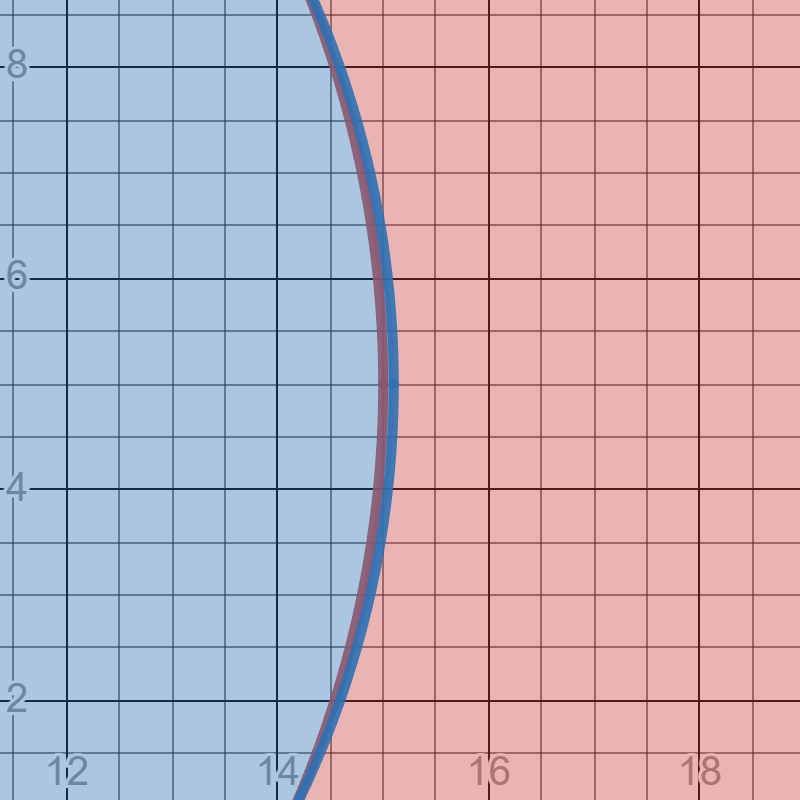
\includegraphics[width=0.5\textwidth]{images/q3_visualizacao.png}
  \caption{Região possível para as soluções da Questão 03}
  \label{fig:q3_valid}
\end{figure}

Os resultados obtidos para a Questão 03 são exibidos em forma tabular na Tabela \ref{tab:q3_results} e graficamente na Figura \ref{fig:q3}. As conclusões obtidas neste caso são similares
às obtidas na Questão 01 e 02.

\begin{table}[htpb]
  \centering
  \begin{tabular}{|l|c|c|c|c|c|c|c|}
    %\cline{2-7}
    \multicolumn{1}{c}{} %\vline
    & 
    \multicolumn{3}{c}{\textbf{Penalidade}} \vline
    & 
    \multicolumn{3}{c}{\textbf{Barreira}} \\%\vline \\
    \hline%\cline{2-5}
    \textbf{Método}
    &
    \textbf{Ponto de mínimo}
    & 
    $\mathbf{n}_{passos}$
    & 
    \textbf{t (s)}
    &
    \textbf{Ponto de mínimo}
    & 
    $\mathbf{n}_{passos}$
    & 
    \textbf{t (s)}
    \\
    Univariante        & $[14.094999, 0.842959]^T$ & 50 & 7.826 &  $[14.095016, 0.842995]^T$ &  10  & 1.607    \\
    Powell             & $[14.095000, 0.842961]^T$ & 12 & 2.007 &  $[14.095023, 0.843006]^T$ &   9  & 0.805    \\
    Steepest Descent   & $[14.095026, 0.843012]^T$ & 43 & 6.768 &  $[14.095157, 0.843304]^T$ &   8  & 1.399    \\
    Fletcher-Reeves    & $[14.095001, 0.842963]^T$ & 14 & 2.507 &  $[14.095009, 0.842980]^T$ &   9  & 1.903    \\
    Newton-Raphson     & $[14.095000, 0.842961]^T$ & 50 & 8.233 &  $[14.095000, 0.842960]^T$ &  13  & 2.355    \\
    BFGS               & $[14.095000, 0.842961]^T$ & 13 & 2.026 &  $[14.095001, 0.842961]^T$ &  12  & 0.518    \\
    \hline
  \end{tabular}
  \caption{Resumo dos resultados obtidos para a Questão 03}
  \label{tab:q3_results}
\end{table}

\begin{figure}[htpb]
  \centering
  \begin{subfigure}[b]{0.32\textwidth}
      \centering
      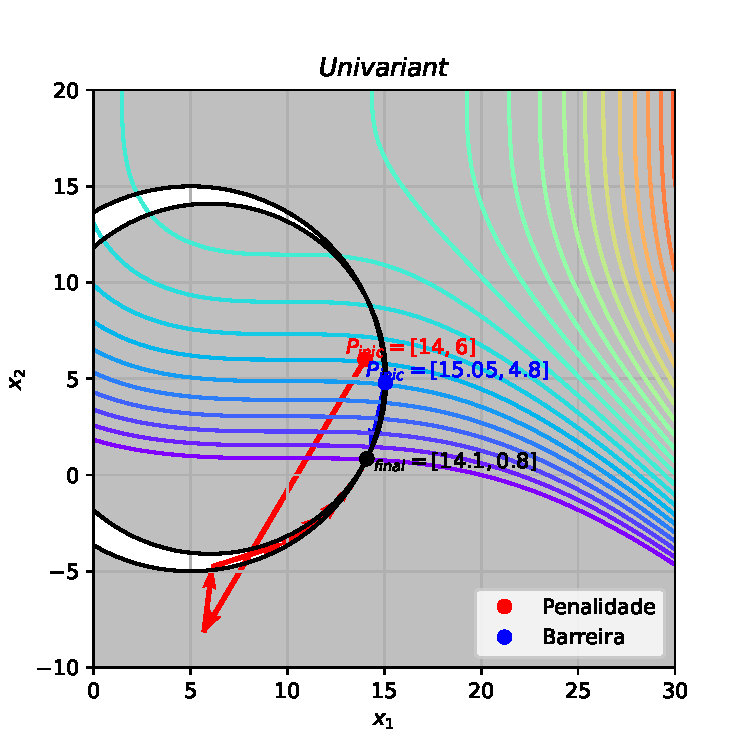
\includegraphics[width=\textwidth]{images/q3_Univariant.pdf}
      \caption{Univariante}
      \label{fig:q3_univariant}
  \end{subfigure}
  \hfill
  \begin{subfigure}[b]{0.32\textwidth}
    \centering
    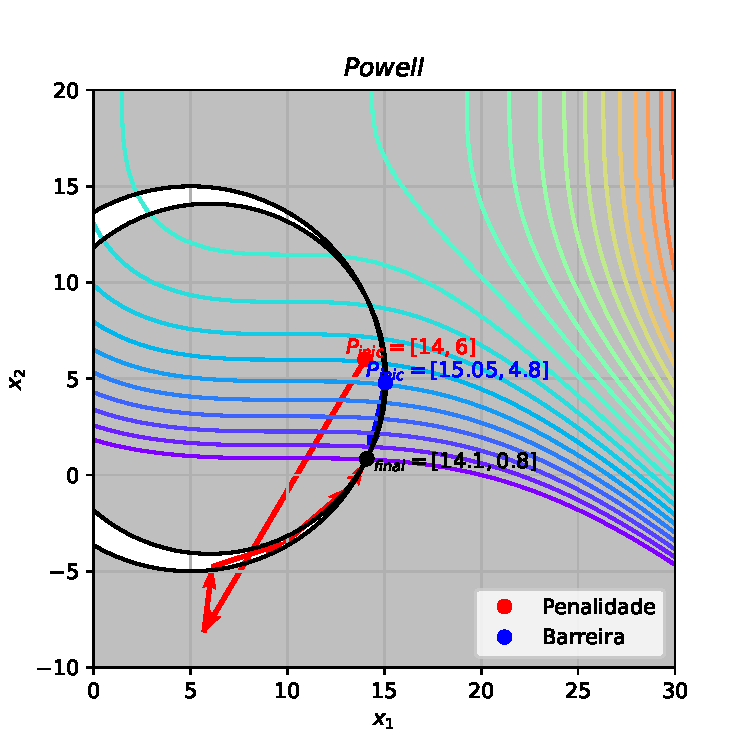
\includegraphics[width=\textwidth]{images/q3_Powell.pdf}
    \caption{Powell}
    \label{fig:q3_powell}
  \end{subfigure}
  \hfill
  \begin{subfigure}[b]{0.32\textwidth}
    \centering
    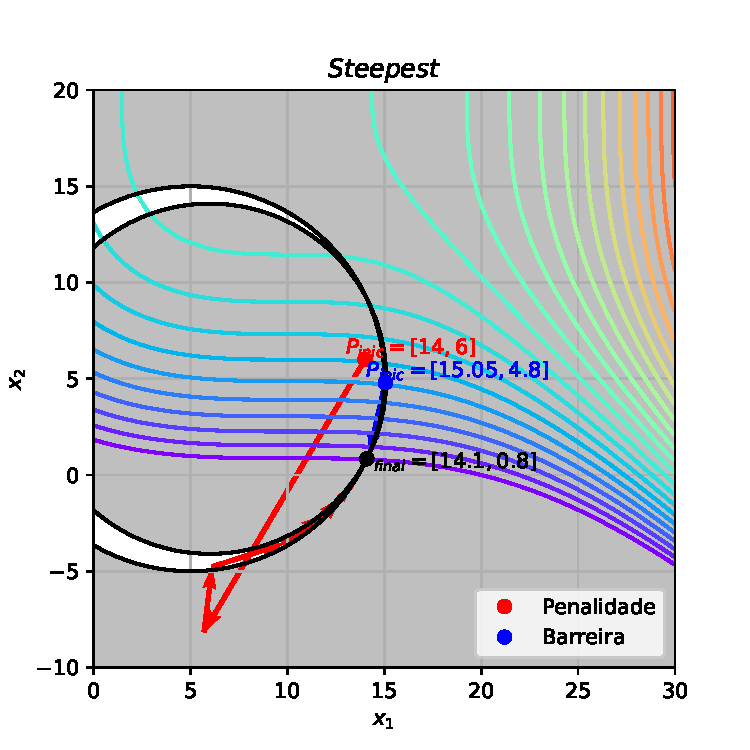
\includegraphics[width=\textwidth]{images/q3_Steepest.pdf}
    \caption{Steepest Descent}
    \label{fig:q3_steepest}
  \end{subfigure}
  \hfill
  \begin{subfigure}[b]{0.32\textwidth}
    \centering
    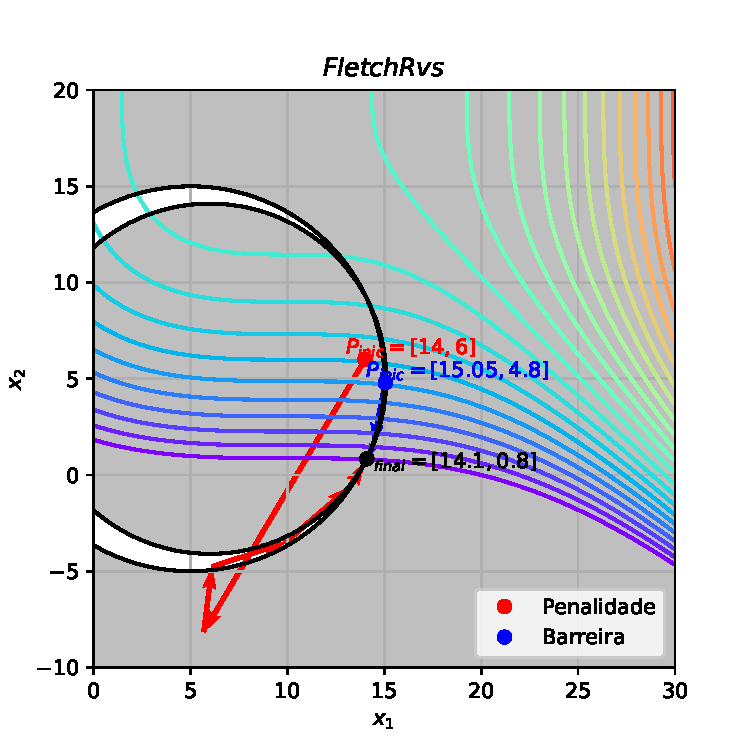
\includegraphics[width=\textwidth]{images/q3_FletchRvs.pdf}
    \caption{Fletcher-Reeves}
    \label{fig:q3_fletchrvs}
  \end{subfigure}
  \hfill
  \begin{subfigure}[b]{0.32\textwidth}
    \centering
    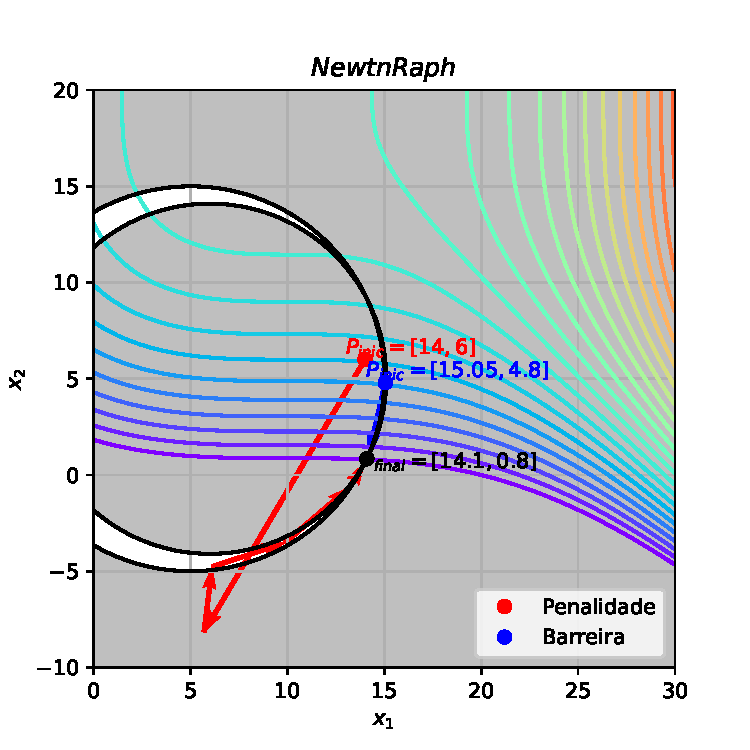
\includegraphics[width=\textwidth]{images/q3_NewtnRaph.pdf}
    \caption{Newton-Raphson}
    \label{fig:q3_newtnraph}
  \end{subfigure}
  \hfill
  \begin{subfigure}[b]{0.32\textwidth}
    \centering
    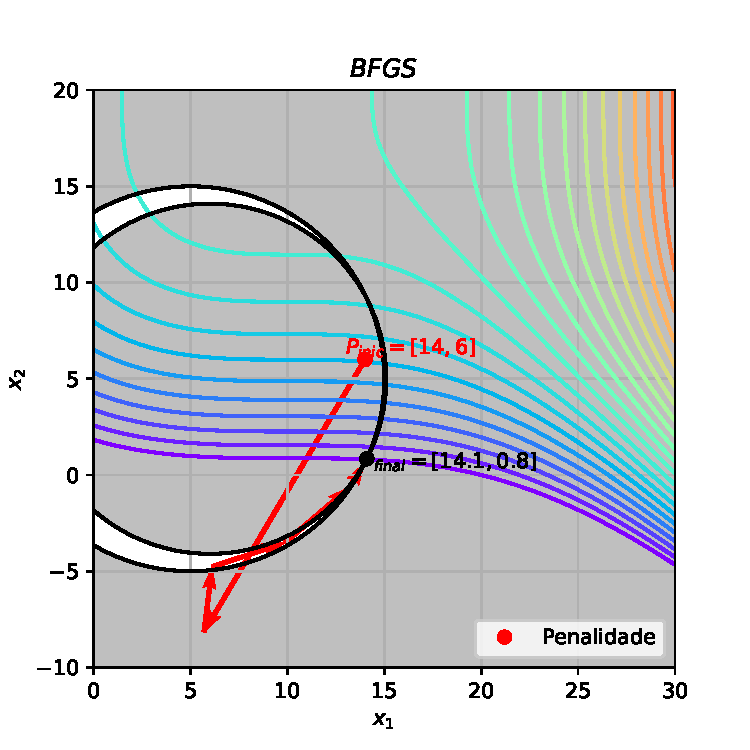
\includegraphics[width=\textwidth]{images/q3_BFGS.pdf}
    \caption{BFGS}
    \label{fig:q3_bfgs}
  \end{subfigure}
     \caption{Resultados gráficos para a Questão 03}
     \label{fig:q3}
\end{figure}

\newpage

\subsection{Questão 04}

O problema proposto para a Questão 04 é o mais complexo da lista em termos de domínio e restrições. Baseado nas equações do enunciado e natureza do problema algumas mudanças no conjunto de restrições foram
feitas, a saber:

\begin{itemize}
  \item As restrições de máximo para $R$ e $t$ foram removidas, dado que a função objetivo já tende a levar para valores menores
  \item Foi criada uma restrição que forçasse $R \ge t$, para evitar soluções em que a espessura fosse superior ao raio
\end{itemize}

Ainda no escopo do enunciado da Questão 04, foi solicitada a seleção de um conjunto de condições iniciais ($\mathbf{x}_0$, $r^0$ e $\beta$). Após alguns testes preliminares, os parâmetros para cada caso
foram selecionados. Os valores usados estão sumarizados na Tabela \ref{tab:q4_initial}.

\begin{table}[htpb]
  \centering
  \begin{tabular}{|l|c|c|c|}
    \hline
    \textbf{Método} & $\mathbf{x}_0$   & $r^0$  & $\beta$          \\
    \hline
    Penalidade      & $[0.2, 0.15]^T$  & $10^5$ & $1\times10^3$    \\
    \hline
    Barreira        & $[0.5, 0.025]^T$ & $10^1$ & $5\times10^{-1}$ \\
    \hline
  \end{tabular}
  \caption{Condições iniciais para a Questão 04}
  \label{tab:q4_initial}
\end{table}

Os resultados obtidos para a Questão 04 estão sumarizados na Tabela \ref{tab:q4_results}. Diferentemente das demais questões neste trabalho, para este caso os métodos de Penalidade e Barreira retornaram valores
diferentes. Comparando os resultados para o método de Barreira, é possível ver que todos os métodos OSR aplicados retornaram pontos relativamente próximos, o que está de acordo com o esperado uma vez que todos
os métodos, em cada passo, buscaram retornar o mínimo da mesma função. O número de passos da otimização OCR para o caso de barreira é evidência também disso.
Já no caso do método de Penalidade, embora a maioria dos métodos OSR tenham retornado essencialmente o mesmo ponto (tendo este ponto, inclusive, um valor de peso a ser minimizado inferior ao ponto obtido na 
Penalidade), vale notar que dois métodos (Steepest e Newton) retornaram pontos muito distintos dos demais. Enquanto o ponto obtido pelo Steepest Descent tem a seu favor ser próximo do obtido pelos métodos quando
aplicado o método da Barreira, o ponto obtido pelo método de Newton é claramente um erro numérico, em que pelas características do método após um passo a convergência foi atingida.

\begin{table}[htpb]
  \centering
  \begin{tabular}{|l|c|c|c|c|c|c|c|}
    %\cline{2-7}
    \multicolumn{1}{c}{} %\vline
    & 
    \multicolumn{3}{c}{\textbf{Penalidade}} \vline
    & 
    \multicolumn{3}{c}{\textbf{Barreira}} \\%\vline \\
    \hline%\cline{2-5}
    \textbf{Método}
    &
    \textbf{Ponto de mínimo}
    & 
    $\mathbf{n}_{passos}$
    & 
    \textbf{t (s)}
    &
    \textbf{Ponto de mínimo}
    & 
    $\mathbf{n}_{passos}$
    & 
    \textbf{t (s)}
    \\
    Univariante        & $[0.067747, 0.005000]^T$ &  3 & 1.337 &  $[0.060146, 0.007125]^T$ &  10  & 3.430    \\
    Powell             & $[0.067748, 0.005000]^T$ &  4 & 1.566 &  $[0.059181, 0.007477]^T$ &   9  & 1.302    \\
    Steepest Descent   & $[0.061623, 0.006629]^T$ &  2 & 1.036 &  $[0.060623, 0.006959]^T$ &  10  & 3.466    \\
    Fletcher-Reeves    & $[0.067747, 0.005000]^T$ &  3 & 1.353 &  $[0.056907, 0.008404]^T$ &   8  & 2.756    \\
    Newton-Raphson     & $[0.037870, 0.028403]^T$ &  1 & 0.531 &  $[0.059698, 0.007286]^T$ &   9  & 3.836    \\
    BFGS               & $[0.071021, 0.005000]^T$ &  5 & 2.369 &  $[0.056884, 0.008414]^T$ &   8  & 1.381    \\
    \hline
  \end{tabular}
  \caption{Resumo dos resultados obtidos para a Questão 04}
  \label{tab:q4_results}
\end{table}

A Figura \ref{fig:q4} corrobora os comentários anteriormente feitos ao mostrar os resultados da Questão 04 de forma gráfica.

\begin{figure}[htpb]
  \centering
  \begin{subfigure}[b]{0.32\textwidth}
      \centering
      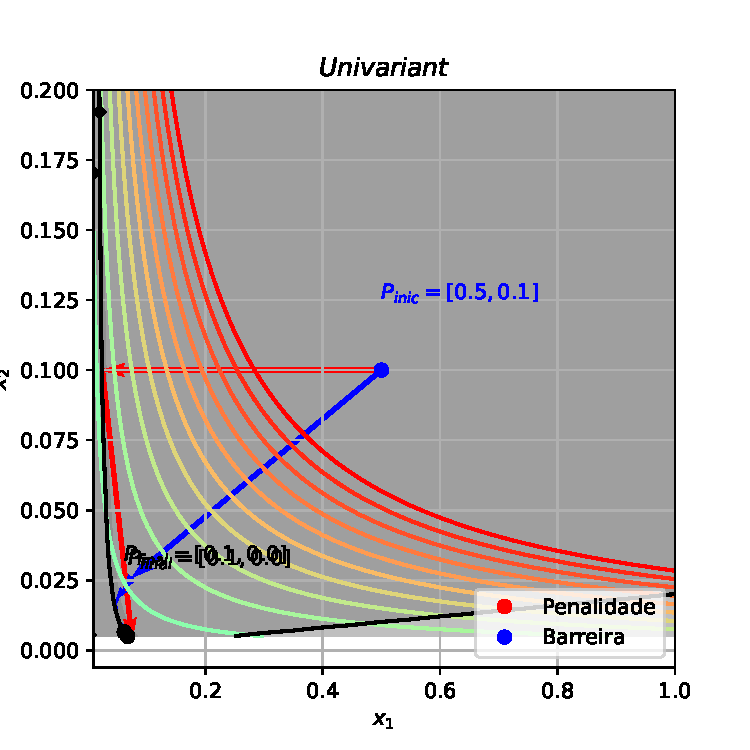
\includegraphics[width=\textwidth]{images/q4_Univariant.pdf}
      \caption{Univariante}
      \label{fig:q4_univariant}
  \end{subfigure}
  \hfill
  \begin{subfigure}[b]{0.32\textwidth}
    \centering
    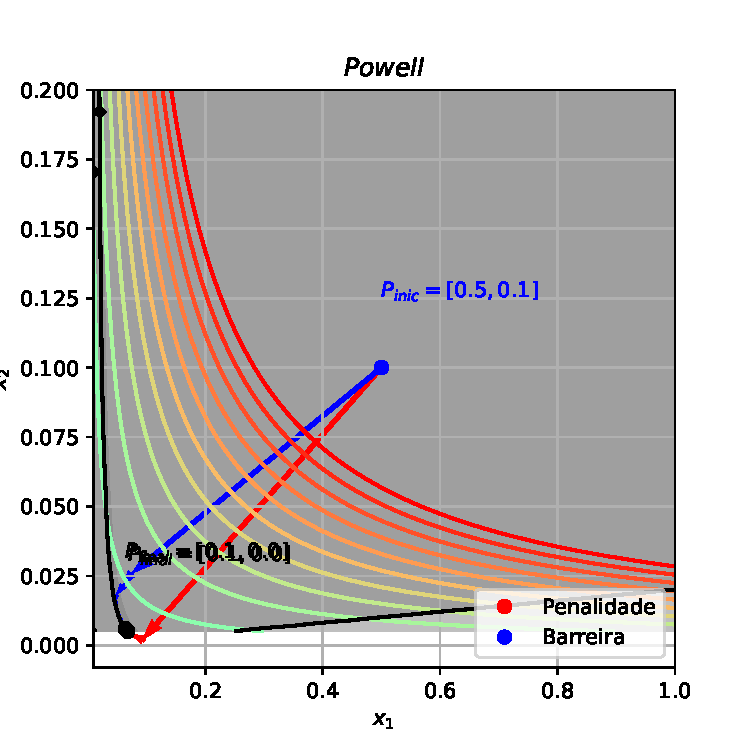
\includegraphics[width=\textwidth]{images/q4_Powell.pdf}
    \caption{Powell}
    \label{fig:q4_powell}
  \end{subfigure}
  \hfill
  \begin{subfigure}[b]{0.32\textwidth}
    \centering
    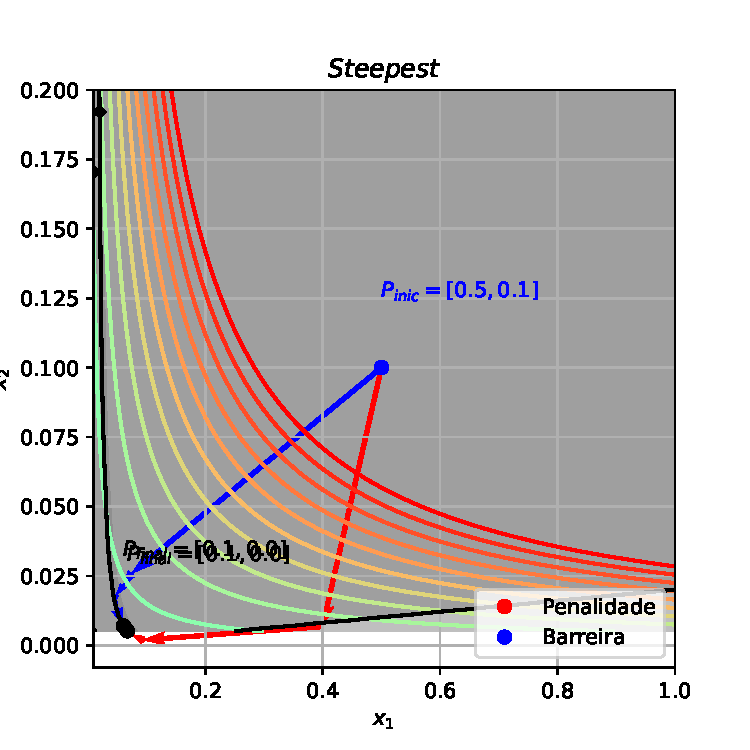
\includegraphics[width=\textwidth]{images/q4_Steepest.pdf}
    \caption{Steepest Descent}
    \label{fig:q4_steepest}
  \end{subfigure}
  \hfill
  \begin{subfigure}[b]{0.32\textwidth}
    \centering
    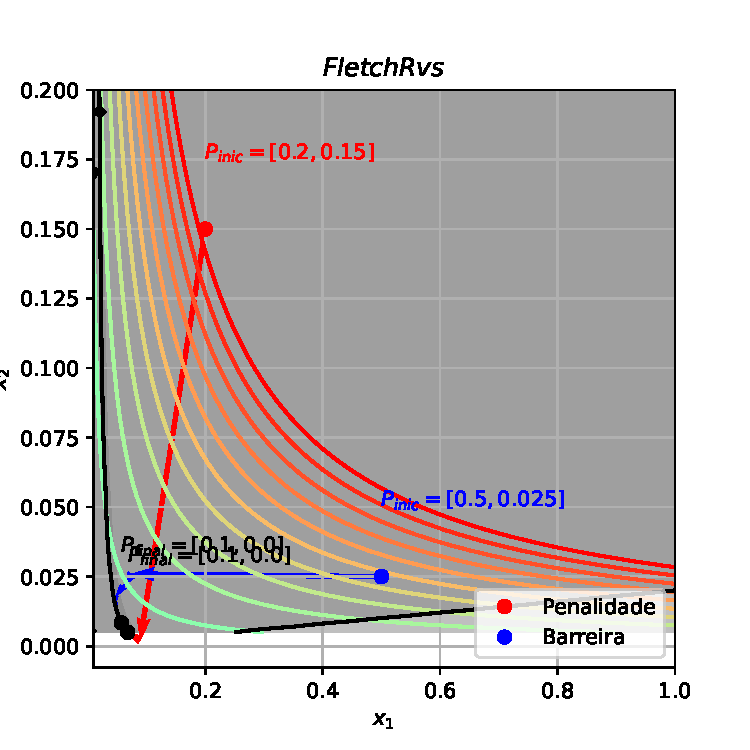
\includegraphics[width=\textwidth]{images/q4_FletchRvs.pdf}
    \caption{Fletcher-Reeves}
    \label{fig:q4_fletchrvs}
  \end{subfigure}
  \hfill
  \begin{subfigure}[b]{0.32\textwidth}
    \centering
    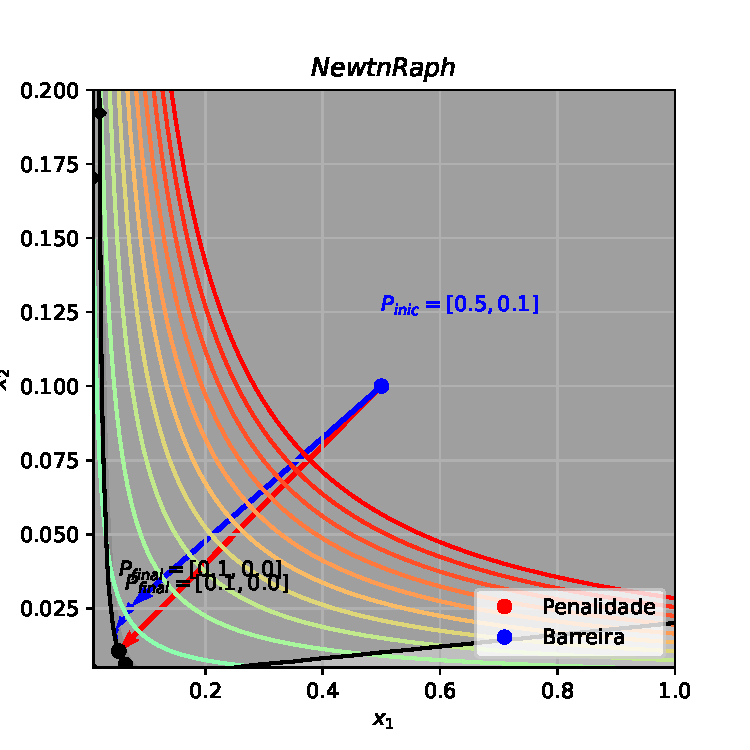
\includegraphics[width=\textwidth]{images/q4_NewtnRaph.pdf}
    \caption{Newton-Raphson}
    \label{fig:q4_newtnraph}
  \end{subfigure}
  \hfill
  \begin{subfigure}[b]{0.32\textwidth}
    \centering
    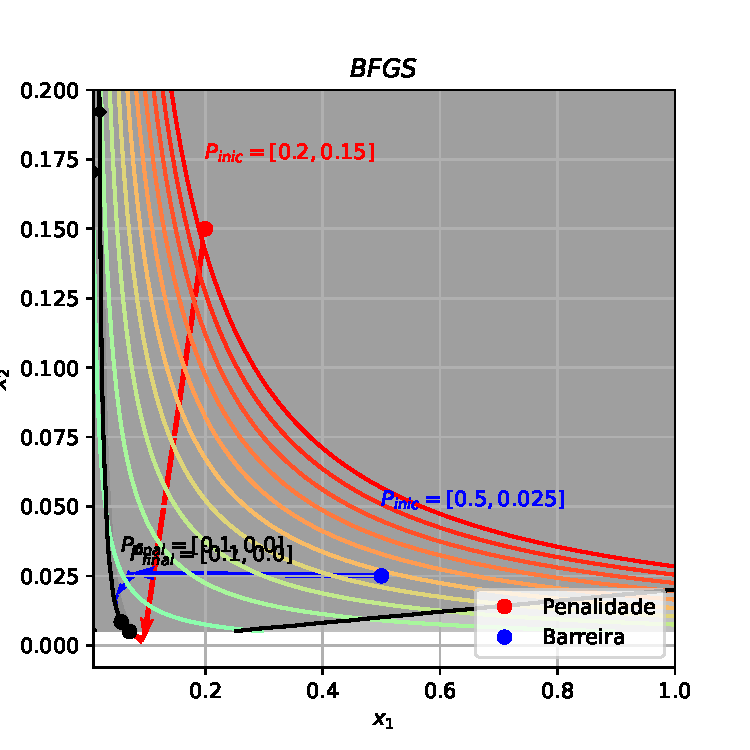
\includegraphics[width=\textwidth]{images/q4_BFGS.pdf}
    \caption{BFGS}
    \label{fig:q4_bfgs}
  \end{subfigure}
     \caption{Resultados gráficos para a Questão 04}
     \label{fig:q4}
\end{figure}



%%%%%%%%%%%%%%%%%%%%%%%%%%%%%%%%%%%%%%%%%%%%%%%%%%%

\bibliographystyle{apalike}
\bibliography{export}

\end{document}